
\documentclass[12pt, a4paper]{report}

% ============================================
% PACKAGES
% ============================================
\usepackage[utf8]{inputenc}
\usepackage[T1]{fontenc}
\usepackage{geometry}
\usepackage{graphicx}
\usepackage{booktabs}
\usepackage{array}
\usepackage{float}
\usepackage{xcolor}
\usepackage{colortbl}
\usepackage{tikz}
\usepackage{pgfplots}
\usepackage{hyperref}
\usepackage{fancyhdr}
\usepackage{titlesec}
\usepackage{tocloft}

% ============================================
% PAGE SETUP
% ============================================
\geometry{
    left=25mm,
    right=25mm,
    top=25mm,
    bottom=25mm
}

% ============================================
% PGFPLOTS CONFIGURATION
% ============================================
\pgfplotsset{compat=1.18}

% ============================================
% COLOR DEFINITIONS
% ============================================
\definecolor{shearpositive}{RGB}{70, 130, 180}    % Steel Blue
\definecolor{shearnegative}{RGB}{220, 20, 60}     % Crimson Red
\definecolor{momentpositive}{RGB}{34, 139, 34}    % Forest Green
\definecolor{momentnegative}{RGB}{255, 140, 0}    % Dark Orange
\definecolor{titleblue}{RGB}{0, 51, 102}          % Dark Blue

% ============================================
% HYPERREF SETUP
% ============================================
\hypersetup{
    colorlinks=true,
    linkcolor=titleblue,
    filecolor=magenta,      
    urlcolor=cyan,
    pdftitle={Beam Analysis Report},
    pdfauthor={FOSSEE Project},
}

% ============================================
% HEADER AND FOOTER
% ============================================
\pagestyle{fancy}
\fancyhf{}
\fancyhead[L]{\small Beam Analysis Report}
\fancyhead[R]{\small \leftmark}
\fancyfoot[C]{\thepage}
\renewcommand{\headrulewidth}{0.4pt}
\renewcommand{\footrulewidth}{0.4pt}

% ============================================
% TITLE FORMATTING
% ============================================
\titleformat{\chapter}[display]
  {\normalfont\huge\bfseries\color{titleblue}}
  {\chaptertitlename\ \thechapter}{20pt}{\Huge}

\begin{document}

% ============================================
% TITLE PAGE
% ============================================
\begin{titlepage}
    \centering
    
    \vspace*{2cm}
    
    % Title
    {\Huge\bfseries\color{titleblue} Structural Analysis Report \par}
    
    \vspace{1cm}
    
    {\LARGE\bfseries Simply Supported Beam Analysis \par}
    
    \vspace{2cm}
    
    % Decorative line
    \noindent\rule{\textwidth}{2pt}
    
    \vspace{2cm}
    
    % Project Information
    {\Large\textbf{Project:} FOSSEE Beam Analysis \par}
    
    \vspace{0.5cm}
    
    {\Large\textbf{Document Type:} Engineering Analysis Report \par}
    
    \vspace{0.5cm}
    
    {\Large\textbf{Analysis Method:} Shear Force \& Bending Moment Analysis \par}
    
    \vspace{3cm}
    
    % Date
    {\large\textbf{Date:} February 03, 2026 \par}
    
    \vfill
    
    % Footer line
    \noindent\rule{\textwidth}{1pt}
    
    \vspace{0.5cm}
    
    {\small Generated using Python and \LaTeX{} \par}
    
\end{titlepage}

% ============================================
% TABLE OF CONTENTS
% ============================================
\tableofcontents
\thispagestyle{empty}
\newpage

% ============================================
% INTRODUCTION
% ============================================
\chapter{Introduction}

\section{Overview}

This report presents a comprehensive structural analysis of a simply supported beam 
subjected to a uniformly distributed load. The analysis includes the calculation and 
visualization of internal forces, specifically the Shear Force Diagram (SFD) and 
Bending Moment Diagram (BMD).

\section{Simply Supported Beam}

A simply supported beam is a fundamental structural element that rests on two 
supports --- a pinned support at one end and a roller support at the other. This 
configuration allows the beam to:

\begin{itemize}
    \item Resist vertical loads through reaction forces at the supports
    \item Freely expand or contract due to thermal effects (roller support)
    \item Rotate freely at both support points
\end{itemize}

\subsection{Beam Configuration}

The beam under analysis has the following configuration:

\begin{figure}[H]
    \centering
    \includegraphics[width=0.85\textwidth]{X:/Participations/FOSSEE/Latex2/simply_supported_beam.png}
    \caption{Simply Supported Beam with Pinned and Roller Supports}
    \label{fig:beam_diagram}
\end{figure}

\textbf{Beam Parameters:}
\begin{itemize}
    \item \textbf{Total Length:} 15.0 meters
    \item \textbf{Left Support:} Pinned support (restricts horizontal and vertical displacement)
    \item \textbf{Right Support:} Roller support (restricts only vertical displacement)
    \item \textbf{Loading:} Uniformly distributed load
\end{itemize}

\section{Analysis Objectives}

The objectives of this structural analysis are:

\begin{enumerate}
    \item Calculate shear forces at critical points along the beam
    \item Calculate bending moments at critical points along the beam
    \item Generate Shear Force Diagram (SFD)
    \item Generate Bending Moment Diagram (BMD)
    \item Identify maximum shear force and bending moment locations
\end{enumerate}

\newpage

% ============================================
% INPUT DATA
% ============================================
\chapter{Input Data}

\section{Force and Moment Data}

The following table presents the calculated values of shear force and bending 
moment at various positions along the beam. These values were obtained from 
structural analysis calculations.

\begin{table}[H]
    \centering
    \caption{Shear Force and Bending Moment Values Along the Beam}
    \label{tab:force_data}
    \vspace{0.5cm}
    \begin{tabular}{|c|c|c|}
        \hline
        \rowcolor{titleblue!20}
        \textbf{Position (x)} & \textbf{Shear Force (V)} & \textbf{Bending Moment (M)} \\
        \textbf{[meters]} & \textbf{[kN]} & \textbf{[kN$\cdot$m]} \\
        \hline
        0.0 & 45.00 & 0.00 \\
        \hline
        1.5 & 36.00 & 60.75 \\
        \hline
        3.0 & 27.00 & 108.00 \\
        \hline
        4.5 & 18.00 & 141.75 \\
        \hline
        6.0 & 9.00 & 162.00 \\
        \hline
        7.5 & 0.00 & 168.75 \\
        \hline
        9.0 & -9.00 & 162.00 \\
        \hline
        10.5 & -18.00 & 141.75 \\
        \hline
        12.0 & 27.00 & 108.00 \\
        \hline
        13.5 & -36.00 & 60.75 \\
        \hline
        15.0 & -45.00 & 0.00 \\
        \hline
    \end{tabular}
\end{table}

\section{Data Interpretation}

From the table above, we can observe:

\begin{itemize}
    \item \textbf{Maximum Positive Shear Force:} 45.00 kN (at x = 0.0 m)
    \item \textbf{Maximum Negative Shear Force:} -45.00 kN (at x = 15.0 m)
    \item \textbf{Maximum Bending Moment:} 168.75 kN$\cdot$m (at x = 7.5 m)
    \item \textbf{Zero Shear Location:} x = 7.5 m (point of maximum moment)
\end{itemize}

\newpage

% ============================================
% SHEAR FORCE DIAGRAM
% ============================================
\chapter{Analysis Results}

\section{Shear Force Diagram (SFD)}

The Shear Force Diagram shows the variation of internal shear force along the 
length of the beam. Positive shear forces are shown in \textcolor{shearpositive}{\textbf{blue}} 
and negative shear forces are shown in \textcolor{shearnegative}{\textbf{red}}.

\begin{figure}[H]
    \centering
    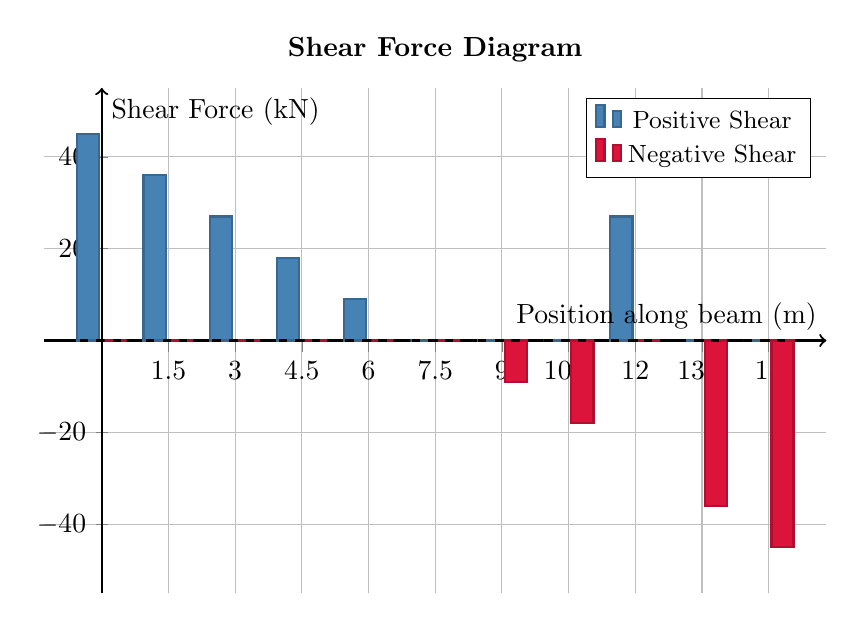
\begin{tikzpicture}
        \begin{axis}[
            width=0.95\textwidth,
            height=8cm,
            xlabel={Position along beam (m)},
            ylabel={Shear Force (kN)},
            title={\textbf{Shear Force Diagram}},
            xmin=-0.5,
            xmax=15.5,
            ymin=-55,
            ymax=55,
            xtick={0.0,1.5,3.0,4.5,6.0,7.5,9.0,10.5,12.0,13.5,15.0},
            grid=both,
            grid style={line width=0.2pt, draw=gray!30},
            major grid style={line width=0.4pt, draw=gray!50},
            axis lines=middle,
            axis line style={->, thick},
            legend style={
                at={(0.98,0.98)},
                anchor=north east,
                draw=black,
                fill=white,
                font=\small
            },
            every axis plot/.append style={thick},
            ybar,
            bar width=8pt,
            enlarge x limits=0.05,
        ]
        
        % Positive Shear Force (Blue)
        \addplot[
            fill=shearpositive,
            draw=shearpositive!80!black,
        ] coordinates {
            (0.0, 45.0)
            (1.5, 36.0)
            (3.0, 27.0)
            (4.5, 18.0)
            (6.0, 9.0)
            (7.5, 0.0)
            (9.0, 0)
            (10.5, 0)
            (12.0, 27.0)
            (13.5, 0)
            (15.0, 0)
        };
        \addlegendentry{Positive Shear}
        
        % Negative Shear Force (Red)
        \addplot[
            fill=shearnegative,
            draw=shearnegative!80!black,
        ] coordinates {
            (0.0, 0)
            (1.5, 0)
            (3.0, 0)
            (4.5, 0)
            (6.0, 0)
            (7.5, 0)
            (9.0, -9.0)
            (10.5, -18.0)
            (12.0, 0)
            (13.5, -36.0)
            (15.0, -45.0)
        };
        \addlegendentry{Negative Shear}
        
        % Zero line
        \draw[black, thick, dashed] (axis cs:-0.5,0) -- (axis cs:15.5,0);
        
        \end{axis}
    \end{tikzpicture}
    \caption{Shear Force Diagram showing the distribution of shear force along the beam}
    \label{fig:sfd}
\end{figure}

\subsection{SFD Observations}

\begin{itemize}
    \item The shear force is maximum positive at the left support
    \item The shear force decreases linearly under uniformly distributed load
    \item The shear force crosses zero at the midpoint of the beam
    \item The shear force is maximum negative at the right support
    \item The slope of the SFD equals the intensity of the distributed load
\end{itemize}

\newpage

\section{Bending Moment Diagram (BMD)}

The Bending Moment Diagram shows the variation of internal bending moment along 
the length of the beam. Positive (sagging) moments are shown in 
\textcolor{momentpositive}{\textbf{green}}.

\begin{figure}[H]
    \centering
    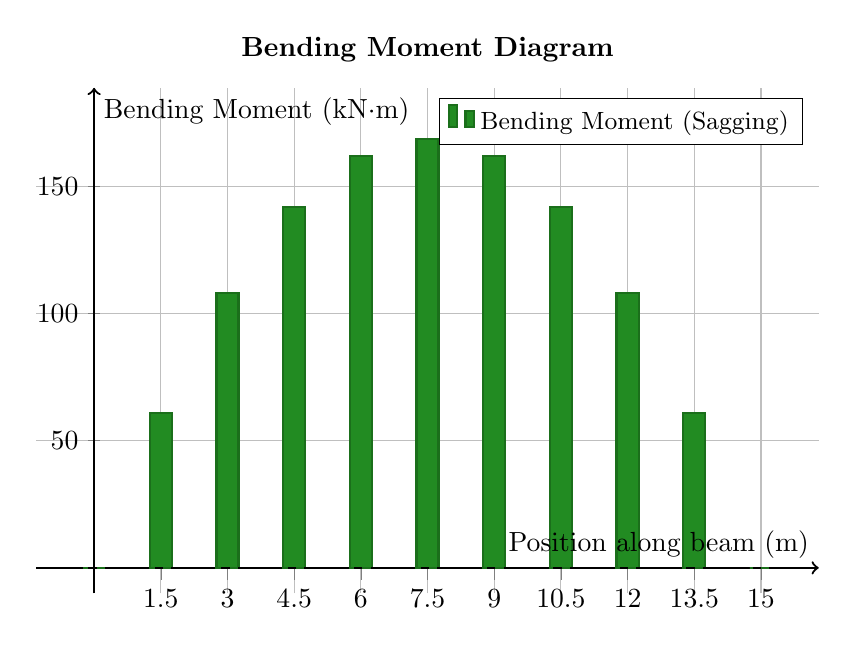
\begin{tikzpicture}
        \begin{axis}[
            width=0.95\textwidth,
            height=8cm,
            xlabel={Position along beam (m)},
            ylabel={Bending Moment (kN$\cdot$m)},
            title={\textbf{Bending Moment Diagram}},
            xmin=-0.5,
            xmax=15.5,
            ymin=-10,
            ymax=188.75,
            xtick={0.0,1.5,3.0,4.5,6.0,7.5,9.0,10.5,12.0,13.5,15.0},
            grid=both,
            grid style={line width=0.2pt, draw=gray!30},
            major grid style={line width=0.4pt, draw=gray!50},
            axis lines=middle,
            axis line style={->, thick},
            legend style={
                at={(0.98,0.98)},
                anchor=north east,
                draw=black,
                fill=white,
                font=\small
            },
            every axis plot/.append style={thick},
            ybar,
            bar width=8pt,
            enlarge x limits=0.05,
        ]
        
        % Bending Moment (Green)
        \addplot[
            fill=momentpositive,
            draw=momentpositive!80!black,
        ] coordinates {
            (0.0, 0.0)
            (1.5, 60.75)
            (3.0, 108.0)
            (4.5, 141.75)
            (6.0, 162.0)
            (7.5, 168.75)
            (9.0, 162.0)
            (10.5, 141.75)
            (12.0, 108.0)
            (13.5, 60.75)
            (15.0, 0.0)
        };
        \addlegendentry{Bending Moment (Sagging)}
        
        % Zero line
        \draw[black, thick, dashed] (axis cs:-0.5,0) -- (axis cs:15.5,0);
        
        \end{axis}
    \end{tikzpicture}
    \caption{Bending Moment Diagram showing the distribution of bending moment along the beam}
    \label{fig:bmd}
\end{figure}

\subsection{BMD Observations}

\begin{itemize}
    \item The bending moment is zero at both supports (simply supported conditions)
    \item The bending moment is maximum at the center of the beam (x = 7.5 m)
    \item Maximum bending moment value: 168.75 kN$\cdot$m
    \item The BMD follows a parabolic curve for uniformly distributed loads
    \item The slope of the BMD at any point equals the shear force at that point
\end{itemize}

\newpage

% ============================================
% CONCLUSION
% ============================================
\chapter{Conclusion}

\section{Summary of Results}

This structural analysis report has presented a comprehensive analysis of a simply 
supported beam with the following key findings:

\begin{table}[H]
    \centering
    \caption{Summary of Critical Values}
    \vspace{0.5cm}
    \begin{tabular}{|l|c|c|}
        \hline
        \rowcolor{titleblue!20}
        \textbf{Parameter} & \textbf{Value} & \textbf{Location} \\
        \hline
        Maximum Positive Shear & 45.00 kN & x = 0.0 m \\
        \hline
        Maximum Negative Shear & -45.00 kN & x = 15.0 m \\
        \hline
        Maximum Bending Moment & 168.75 kN$\cdot$m & x = 7.5 m \\
        \hline
    \end{tabular}
\end{table}

\section{Design Recommendations}

Based on the analysis results, the following recommendations are made for the 
design of this simply supported beam:

\begin{enumerate}
    \item \textbf{Shear Reinforcement:} Provide adequate shear reinforcement near 
          the supports where shear forces are maximum.
    
    \item \textbf{Flexural Reinforcement:} Provide maximum flexural reinforcement 
          at the midspan where the bending moment is maximum.
    
    \item \textbf{Deflection Check:} Verify that the beam deflection under service 
          loads is within acceptable limits.
    
    \item \textbf{Support Design:} Design the supports to safely transfer the 
          reaction forces to the foundation.
\end{enumerate}

\section{Report Generation}

This report was automatically generated using:
\begin{itemize}
    \item Python for data processing and LaTeX generation
    \item TikZ/PGFPlots for vector graphics diagrams
    \item \LaTeX{} for professional document formatting
\end{itemize}

\end{document}
